%% intro.tex
\chapter{Background and Literature Review}
%%%%%%%%%%%%%%%%%%%%%%%%%%%%%%%%%%%%%%%%%%%%%%%%
\label{chap:backGround}
This chapter reviews methods for monolingual and multilingual POS tagging. It provides background knowledge that is necessary for the next chapters. Monolingual POS tagging aims at building a tagger for a single language, and it does not take into account the relationship with other languages. Monolingual POS tagging is language-specific, which might used languages rules/heuristics to improve performance. Multilingual POS tagging, on the other hand, favoring a language-independent approach. It takes into account the relation between languages and aims at building taggers for many languages. More specifically, multilingual taggers build a tagger for one language based on data from other languages. Monolingual POS taggers exploit supervised, semi-supervised or unsupervised methods depending on the availability of data. Multilingual POS tagger, in contrast, is more focused on unsupervised methods with extra information from other (resource-rich) languages.  

\section{Monolingual POS Tagger}
As mentioned before, POS tagger has gained much attention in the past and has achieved great success. Many algorithms for POS tagging have been developed over time. In this section, we are going to review some of them. Moreover, all POS taggers can be divided into 3 categories: \textit{supervised, unsupervised and semi-supervised}. Current best taggers for English are showed in Table \ref{tab:eng_state_of_the_art}\footnote{http://aclweb.org/aclwiki/index.php?title=POS\_Tagging\_(State\_of\_the\_art)}. All these taggers used the Penn Treebank Tagset~\cite{PenTreeBank} and are evaluated on the Wall Street Journal (WSJ) data set. The performance is measured based on per-token accuracy. Moreover, the accuracy for all tokens and unknown tokens are also given. As expected, all the best systems use some of the label data as training data in supervised or semi-supervised style. Moreover, some systems also used external resources to handle OOV or improve the accuracy. 

\begin{table}
  \centering
    \begin{tabular}{p{4cm}p{6cm}cc}

    \multicolumn{1}{c}{\textbf{System name}} & \multicolumn{1}{c}{\textbf{Short description}} & \multicolumn{1}{c}{\textbf{All tokens}} & \multicolumn{1}{c}{\textbf{OOV}} \\
\hline
    TnT  & Hidden markov model & 96.46\% & 85.86\% \\
    %\hline
    MElt  & MEMM with external lexical information & 96.96\% & 91.29\% \\
    %\hline
    GENiA Tagger** & Maximum entropy cyclic dependency network & 97.05\% & NA \\
    %\hline
    Maxent easiest-first & Maximum entropy bidirectional easiest-first inference & 97.15\% & NA \\
    %\hline
    SVMTool & SVM-based tagger and tagger generator & 97.16\% & 89.01\% \\
    %\hline
    Stanford Tagger 1.0 & Maximum entropy cyclic dependency network & 97.24\% & 89.04\% \\%\hline
    Stanford Tagger 2.0 & Maximum entropy cyclic dependency network & 97.29\% & 89.70\% \\%\hline
    Stanford Tagger 2.0 & Maximum entropy cyclic dependency network & 97.32\% & 90.79\% \\%\hline
    SCCN  & Semi-supervised condensed nearest neighbor & 97.50\% & NA \\%\hline

    \end{tabular}
  \caption{List of best English taggers (all $>96\%$ on WSJ test set)}
  \label{tab:eng_state_of_the_art}
\end{table}


\subsection{Supervised}
In this part we review some supervised tagging algorithms. Each algorithm is in a different style, that is, \textit{rule based, probabilistic, feature based} and some \textit{other approaches}.  

\subsubsection{Transformation Based Tagging - a rule based approach} 
Transformation base tagging (TBT) \cite{Brill95transformation} uses rules to tag. For example, a rule could be, ``A word after determiner is Noun" or ``a/an/the are determiner". These rules are acquired from training data. So, basically, TBT contains two components, the \textbf{learner} and the \textbf{tagger}. The learner learns transformation rules from training data. The tagger uses these rules to tag. 

\paragraph{The learner} Steps for the learner are visualized in Figure \ref{fig:tbt_learner}. More detail is as follows:
 
\begin{itemize}
\item Strip the tag off the annotated data but keep the original data to evaluate. 
\item Initialize label for stripped data by some simple method such as, using frequency or any available tagger. 
\item Start with an empty set of selected rule $S$. 
\item Repeat until the stopping criterion is applied. Each iteration, the input are the truth data, pool of possible rules and intermediate data from previous iteration. For each rule $r$ in pool of rules, compute its contribution as follow:

\parbox{\linewidth}{$$contrib(r) = c_{improved}(r) - c_{worsened}(r) $$ }
where $c_{improved}(r)$ is the number of correct items which originally incorrectly tagged and $c_{worsened}(r)$ is the number of incorrect items (originally  correctly tagged) after  applying rule $r$. Afterward, they select a rule \textit{r} which has the biggest contribution $contrib(r)$ and add to the final set of selected rules $S$. The pool of rules is acquired automatically or manually. Rules are designed in the form, ``\textit{change the tag from A to B / condition}". For example, the rule ``\textit{NN $\rightarrow$ NNS / preceded by NN VBP}", say: change the tag at current position from \textit{NN} to \textit{NNS} if two previous tags are \textit{NN} and \textit{VBP}. This step stop when no improvement can be made or the improvement less than a threshold. 
\item Output set of rule \textit{S}
\end{itemize}

\begin{figure}
\centering
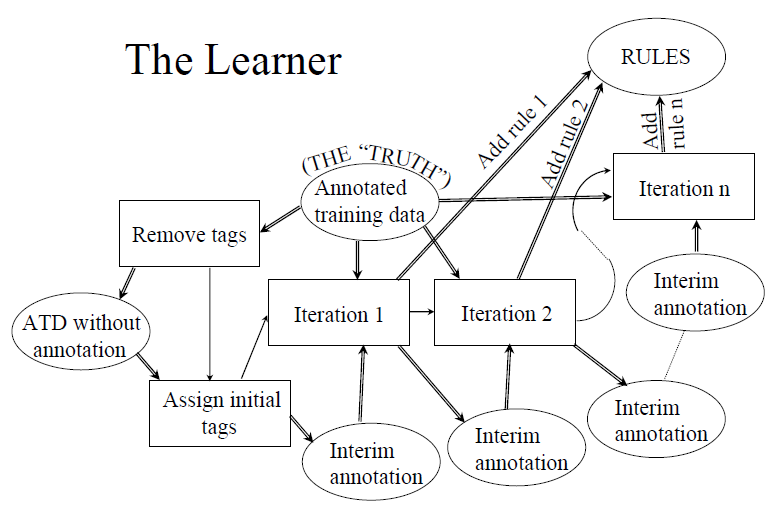
\includegraphics[scale=0.6]{Figures/TBT_learner}
\caption{Learner component of TBT }
\label{fig:tbt_learner}
\end{figure}

\paragraph{The Tagger} The input for tagger is unlabeled data and set of rules $S$ from the learner. Steps for the tagger are straightforward. 
\begin{itemize}
\item Initialize label for lexical items in the same way as the learner did.
\item Loop for all the rules. For each rule \textit{r}, apply this rule to the whole intermediate to change some tag. 
\item The last intermediate data is the output. 
\end{itemize}

TBT is one of the oldest and a very straightforward algorithm, however, it might be used to improve the accuracy of the original tagger. That is, use the original tagger to initialize the learner. \namecite{vietnameseTagger} initialize the learner by using an available English tagger. They also exploit external information from Vietnamese-English parallel data. The English tagger's performance is significantly improved, accuracy improved from 95.4\% to 97.5\% (absolute). 

The Brill Tagger \cite{Brill95transformation} is one of the implementation of transformation base learning. TBT is straightforward but, the learning and tagging is quite slow. Performance of TBT largely depends on having pool of rule templates which are developed by linguist or acquired from machine learning algorithm on annotated corpus. Moreover, compared with other taggers, this approach has rather poorer performance. 

\subsubsection{Hidden Markov Model - a probabilistic approach}
The idea of Hidden Markov Model (HMM) tagger is very similar to noisy channel or translation model in statistical machine translation. The difference is that the output is not a target text but a sequence of tags. Given a sentence which is a sequence of words $W = w_1w_2w_3....w_n$, we need to find the corresponding sequence of tags $T = t_1t_2t_3..t_n$ which maximizes the following probability. 

$$ Tags = \operatorname*{arg\,max}_{t_i} \;P(t_1t_2t_3..t_n|w_1w_2w_3....w_n) = \operatorname*{arg\,max}_{T} \;P(T|W)$$
According to Bayes' rules 
$$P(T|W) = \frac{P(W|T) \times P(T)}{ P(W)} $$
Since we're choosing tags, $P(W)$ is not considered, therefore 
$$Tags = \operatorname*{arg\,max}_{T}\; P(T|W) = \operatorname*{arg\,max}_{T}\; P(W|T) \times P(T) $$
where 
$$ P(W|T) \times P(T)=P(w_1w_2..w_n|t_1t_2..t_n) \times P(t_1t_2..t_n)$$
According to chain rule
$$ P(W|T) \times P(T) = P(w_1|t_1t_2..t_n)\times P(w_2|t_1t_2..t_n) \times P(w_3|t_1t_2..t_n) \times .... \times P(w_n|t_1t_2..t_n) \times $$
$$ P(t_n|t_1..t_{n-1}) \times P(t_{n-1}|t_1..t_{n-2}) \times ...\times P(t_1) $$
\begin{equation}
\label{equa:chainRule}
= \prod_{i=1}^{n} P(w_i|w_1t_1....w_{i-1}t_{i-1}) \times P(t_i|w_1t_1....w_{i-1}t_{i-1})
\end{equation}
With the assumption that the probability of word doesn't depend on the context but only on current tag, we have: 
\begin{equation}
\label{equa:assump1}
P(w_i|w_1t_1....w_{i-1}t_{i-1})  \approx P(w_i|t_i)
\end{equation}
With the assumption that the choice of tag depends on limited history (for example bigram context), we have: 
\begin{equation}
\label{equa:assump2}
P(t_i|w_1t_1....w_{i-1}t_{i-1}) \approx P(t_i|t_{i-1})
\end{equation}
From equation (\ref{equa:chainRule}), (\ref{equa:assump1}) and (\ref{equa:assump2}):
\begin{equation}
\label{equa:hmmFinalEquation}
Tag\; Sequence = \operatorname*{arg\,max}_{T} \; P(W|T) \times P(T) \approx \operatorname*{arg\,max}_{t_i} \; \prod_{i=1}^{n} P(w_i|t_i) \times P(t_i|t_{i-1})
\end{equation}

\begin{figure}
\centering
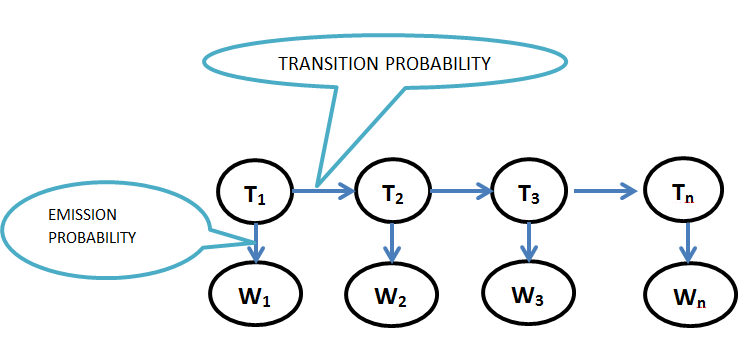
\includegraphics[scale=0.5]{Figures/HMM_tagger}
\caption{Emission and transition probabilities. $W_i$ is a word and $T_i$ is a tag}
\label{fig:hmmTagger}
\end{figure}

$ P(w_i|t_i) $ is called the \textit{emission probability} and $P(t_i|t_{i-1})$ is called the \textit{transition probability} as shown in Figure \ref{fig:hmmTagger}. We estimate these probabilities from training data and then smooth them using method such as interpolation~\cite{REINSCH1967} or Good Turing~\cite{Gale94goodturing}. Smoothing is needed because training data might not cover everything that appears in test data. 

HMM tagging is not as trivial as transformation based tagging. The straightforward tagging solution is that we list all possible tag sequences and calculate the probability of each sequence based on equation \ref{equa:hmmFinalEquation}. The result is the tag sequence that gave the highest probability. However, this solution is not realistic because of the exponential complexity. Therefore, people use dynamic programming algorithms such as Viterbi~\cite{Ryan:1993} or beam search~\cite{beamsearch}.

TNT~\cite{TNTTagger} is an implementation of HMM approach which uses trigram tag model, i.e. $P(t_i|t_{i-1}t_{i-2})$ instead of bigram tag model as mentioned above. Back to Table \ref{tab:eng_state_of_the_art} (page \pageref{tab:eng_state_of_the_art}) , we can see that TNT performs well and achieves comparable result with the state-of-the-art tagger.

\subsubsection{Maximum Entropy - a feature based approach}
We aim at maximizing the following probability 
$$ \operatorname*{arg\,max}_{t_i} \;P(t_1t_2t_3..t_n|w_1w_2w_3....w_n) = \operatorname*{arg\,max}_{T} \;P(T|W)$$
HMM tried to maximize the joint probability $P(W,T)$
$$ \operatorname*{arg\,max}_{T} \;P(T|W) = \operatorname*{arg\,max}_{T} \;P(W|T) \times P (T) = \operatorname*{arg\,max}_{T} \;P(W,T) $$
Maximum Entropy Tagging (MaxEnt)~\cite{maximumEntropy} directly targets maximizing conditional probability $P(T|W)$. 
The disadvantage of HMM tagging is that it cannot incorporate many source of evidence from the text. It just uses lexical and tag information which denoting in emission and transition probability. The MaxEnt model resolves this disadvantage. We can embed as much information as we want in to this MaxEnt model. These information might vary from position, lexical, tag, global document and so forth. Each of these pieces of information are call features. This is the reason why Maximum Entropy tagger belongs to the feature based approach. Formally, a feature is defined as: 

\[
 f_i(C,t) =
  \begin{cases}
   1 & \text{if } context\; C\;is\; satisfied   \\
   0  & otherwise
  \end{cases}
\]

The feature could be complicated or simple, but a feature always in the form, context $C$ and tag $t$. For example a feature ``\textit{suffix = -ing and tag =  VBG}" can be denoted as 
\[
 f_i(C,t) =
  \begin{cases}
   1 & \text{if } \;suffix = \; -ing \; \& \; t = VBG   \\
   0  & otherwise
  \end{cases}
\]\\
The model using these features has to obey the \textbf{constraints}, that is, expected value of feature $f_i$ which is $E_p f_i$ must comply with training data. 
$$E_p f_i = E_{p'}f_i$$
Where 
$$E_{p'}f_i = \frac{1}{N} \sum_{j=1}^{N}f_i(C_j,t_j)$$
$E_{p'}f_i$ is the expected value of feature $f_i$ which is derived from training data ($C_1,t_1$),($C_2,t_2$) .. ($C_n,t_n$). This list can be derived easily from manually annotated data. Apply Lagrangian Multipliers on these constraints, we derived MaxEnt model which has the form as follows:
\begin{equation}
\label{equa:loglinearMaxEnt}
p(t|C) = \frac{1}{Z(C)} exp\Big( \sum_{i=1}^{n}\lambda_if_i(C,t)    \Big)
\end{equation}
Where 
\begin{itemize}
\item $f_i$ is a feature function as defined above 
\item $C$ is the context, t is tag 
\item $Z(C)$ is the normalization factor to ensure proper distribution probability. 
\item $\lambda_i$ is the weight for features $f_i$
\end{itemize}
The more common name for this model is ``log-linear model". We use Generalized Iterative Scaling (GIS)~\cite{Darroch1972} to estimate $\lambda_i$. The value of  $\lambda_i$ shows the importance of feature $f_i$. This value has to obey the \emph{constraints} applied for feature $f_i$. The GIS algorithm is shown in Algorithm \ref{alg:findLambda}.
\begin{algorithm}
\caption{Finding $\lambda_i$}
\label{alg:findLambda}
\begin{algorithmic} 
\STATE $\lambda_i^{(0)} \leftarrow 0$
\WHILE{$not\;convergence$}
\STATE $C \leftarrow max_{C,t} \sum_{i=1}^{n} f_i(C,t)$
\STATE $\lambda_i^{(t+1)} \leftarrow \lambda_i^t + \frac{1}{C}log\frac{E_{p'}f_i}{E_{p^{(t)}}f_i}$
\ENDWHILE
\end{algorithmic}
\end{algorithm}

It is very important to notice that the constraints cannot uniquely define the model in Equation (\ref{equa:loglinearMaxEnt}). So, from all models that satisfy constraints, we choose a model that \textit{maximizes entropy}, that is, as uniform as possible. Moreover, tag probability truly depends on the context which is described by features, therefore: 
\begin{equation}
\label{equa:finalMaxEnt}
Tag\; Sequence = \operatorname*{arg\,max}_{T} \;P(T|W) = \operatorname*{arg\,max}_{T}; P(T|C) \approx \operatorname*{arg\,max}_{t_i};\prod_{i=1}^{n} p(t_i|C_i)
\end{equation}
Finally, the most probable sequence of tags (\textit{result tag sequence}) is obtained by performing beam search~\cite{beamsearch} or Viterbi~\cite{Ryan:1993} algorithms to maximize equation (\ref{equa:finalMaxEnt}). 

The most common implementation of MaxEnt tagger uses features from two words back and ahead, the current word, and two tags back. That is, context C = $(w_{i-2},t_{i-2}, w_{i-1}, t_{i-1}, w_i, w_{i+1}, w_{i+2})$. Features can be anything from this context. Therefore, the number of features can be numerous and degrade the performance. Effective implementation always uses some heuristic methods to limit the number of features. Stanford Maximum Entropy tagger~\cite{Toutanova:2003} is one of notable such implementation. From Table \ref{tab:eng_state_of_the_art} (page \pageref{tab:eng_state_of_the_art}), we can see that aside from Stanford MaxEnt, there are many other systems i.e. GENiA Tagger~\cite{Toutanova03} or Maxent easiest-first~\cite{Tsuruoka:2005}  exploit MaxEnt idea and acquire very good result. This is somehow understandable because MaxEnt has the power to incorporate all features. In that way, we capture all evidence that could help to predict tags.  
% How to construct features .

\subsubsection{Other algorithms}
Apart from the above mentioned approaches (rule based, probabilistic, feature based), there are other approaches for supervised POS taggers. 

The \textit{classifier base approach} is one of those. They build a classifier based on machine learning algorithms such as Naive Bayes, Decision Tree, kNN or more advanced methods: Support Vector Machines (SVM) or Conditional Random Fields (CRF) and so forth. Each lexical item (word) is converted into features, then a classifier is  trained on this data. The test data is also converted into features. We run the classifier on test data and produce tag labels. Steps for classifier approach are described in Figure \ref{fig:machineLearning}. Back to Table \ref{tab:eng_state_of_the_art} (page \pageref{tab:eng_state_of_the_art}), SVMtool~\cite{svmtool} implement SVM machine learning algorithm performs very well on Wall Street Journal (WSJ) data set.
\begin{figure}
\centering
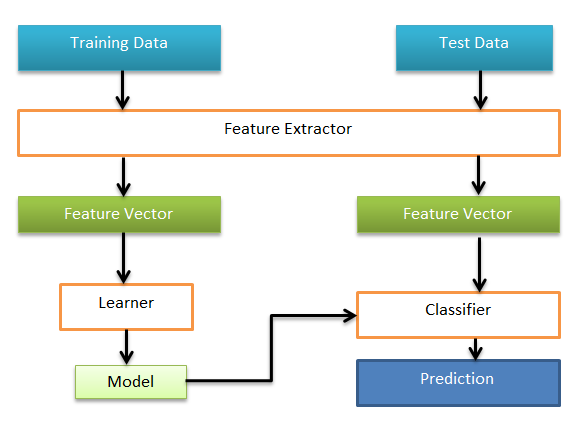
\includegraphics[scale=0.6]{Figures/MachineLearning}
\caption{Steps to build a classifier}
\label{fig:machineLearning}
\end{figure}

\textit{Parsing approach} exploits the idea of building a constituency parse tree as in Figure \ref{fig:parsingTagging}. Afterward, we need to track down the rules to determine tags. For example, from rule NP $\rightarrow$ DT NN, we extract ``\textit{a}" (DT) and ``\textit{fly}" (NN). However, parsing task is more difficult than tagging and actually uses information from tagging processes. Nevertheless, parsing could be very helpful for tagging especially in the case where disambiguation needs a long range syntactic information as in Chinese or Japanese. Traditionally, a constituency parser is built from a tree bank using algorithms such as shift-reduce parsing \cite{shiftReduce}. Modern approach does POS tagging and parsing at the same time in an incremental way \cite{ParsingAndTagging}. 
\begin{figure}
\centering
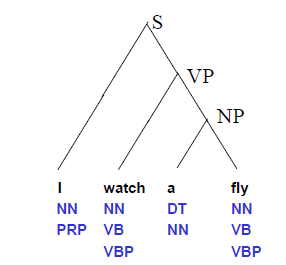
\includegraphics[scale=0.8]{Figures/Constituency_parsing}
\caption{Constituency Parse Tree}
\label{fig:parsingTagging}
\end{figure}

\subsection{Unsupervised}
Unsupervised tagging does not use any labeled data for training. There are several well-known methods for unsupervised tagging.  
\subsubsection{Clustering}
Words having the same syntactic properties are grouped into the same group (cluster). It is believed that words in the same cluster are likely to have the same POS tag. The first issue a clustering tagger has to tackle is \textit{measuring syntactic similarity}. That is if each word is a vertex in a graph, and the weight of edges between vertexes is the syntactic similarity, then words which have the same POS label must be close to each other. Normally, similarity measurement algorithm is based on nearby content words. For example, in two sentences ``\textit{He bought a pair of shoes}" and ``\textit{He ate a banana}". Two words ``\textit{bought}" and ``\textit{ate}" are surrounded by ``\textit{He}" and ``\textit{a}", therefore ``\textit{buy}" and ``\textit{eat}" are likely to have the same POS tag. \namecite{disPOSTagging} proposes to use distributional similarity for measurement. This approach is based on the hypothesis that, ``we can understand a word by looking at its neighbor feature words". Afterward, a word is displayed as vectors of feature words. To compensate for the frequency effects, the weight for each feature word is calculated using a method such as tf.idf~\cite{tfidf}. \namecite{disPOSTagging} considers the top $n$ most frequent words as feature words. A word is displayed as: 
$$\overrightarrow{word A} = (w_1,w_2,w_3......w_n)$$
where $w_i$ is the weight of the $i^{th}$ feature word and $w_i$ = 0 if that feature word does not appear in the context of current $word A$. The similarity between two words is the cosine similarity between the corresponding vectors. 

Another problem with clustering tagger is \textbf{determining the number of clusters}. Defining that number beforehand might not be a good solution. We might force the algorithm to separate coherent cluster or to join unrelated one. On the other hand, letting the algorithm choose when to stop could result in a too specific or too general cluster. 

\textbf{Evaluation} is also another major consideration. Normally, clustering algorithms are evaluated based on the perplexity (or entropy) of the cluster. In the case of tagging, we are expecting that all words in the same cluster have the same tag. Therefore, the lower the perplexity, the better. However, is it what we are looking for? The answer is no, we want to compare with gold standard test data to know the tagging performance. \citeauthor{ManyToOneEvaluate} (2007) suggested a \textit{many-to-one} evaluation. The induced tag for each cluster is the most frequent tag of the items in the cluster, consulting the gold standard data. However, there are cases where two clusters have the same tag. To resolve this issue,\textit{ one-to-one} evaluation puts the restriction that each gold tag corresponds to only one cluster. Normally, it is done by greedy matching, which aims at maximizing  accuracy. Nevertheless, the number of clusters and gold tags are likely to be different. In that case, some clusters or gold tags will not be matched. However, both \textit{many-to-one} and \textit{one-to-one} evaluation schemes require gold data to find the most appropriate tag for each cluster. This is a chicken-and-egg problem since if we have gold data then we don't need to take an unsupervised approach. Besides, we can also use some heuristic method to determine the tag for each cluster such as cluster size (eg, the biggest cluster is Noun). 

UnsuPOS\footnote{http://wortschatz.uni-leipzig.de/\textasciitilde cbiemann/software/unsupos.html} \cite{unSupPOSClustering} is an implementation of a clustering tagger. He divides words into two partitions: high and medium frequency words, medium and low frequency words. In each partition, he builds a different graph using a different similarity measurement. For high and medium frequency words, he uses distributional similarity as mentioned above. For the other partition, he calculates similarity between two words based on how many \textit{direct} neighbors they have in common. The edge is made between words (vertex) if the weight is higher than a threshold. Afterward, the Chinese Whispers~\cite{chineseWhisper} clustering algorithm is performed on both graphs. Steps for Chinese Whispers are simply as follows: (1)~each node is assigned to a cluster; (2)~sort the nodes in an random order; (3)~join node to it most popular neighborhood where popularity is defined as the total weight of inside nodes; (4)~repeat (3) until the number of cluster reaches the fix point. 


Thereafter, on each partition, there is a set of clusters. It is worth noticing that there are many words in common (medium frequency words) between clusters. Then, \namecite{unSupPOSClustering} merges these two sets into a single set. Again, each cluster is considered as a vertex and the number of common words is the weight between vertexes. Chinese Whisper is applied  again to acquire final clusters. Every word inside a cluster has cluster ID as the tag label. Finally, he build a tagging model using a trigram HMM. 

Unsupervised tagging using a clustering algorithm is useful since it provides the first overview about syntactic categories of lexical items. In reality, it is usually used with other applications, for example, \namecite{semiSuPOSCondense} uses unsupervised tagging information as the feature to build another tagger. 

\subsubsection{HMM unsupervised tagging}
\label{hmmUnsup}
In a supervised HMM tagger, we estimate emission probability $p(w_i|t_i)$ and transition probability $p(t_i|history)$ from the labeled training data. In the unsupervised style, these two probabilities are estimated using the Baum-Welch~\cite{BaumWelch} algorithm, which is a variant of the \textit{Expectation Maximization (EM)} algorithm. It means that Baun-Welch can only output the local best but not the global optimal solution. Baum-Welch makes use of forward and backward algorithms~\cite{forwardBackward}. It uses the sequence of observations and outputs the most likely parameters (emission and transition probability) for the HMM. Roughly speaking, the steps for Baum-Welch are described in Algorithm \ref{alg:baumWelch}. 
% Steps for baun-welch 
\begin{algorithm}
\caption{Baum-Welch algorithm}
\label{alg:baumWelch}
\begin{algorithmic} 
\STATE Initialize emission probability $P_Y$
\STATE Initialize transition probability$P_S$
\WHILE{$not\;convergence$}
\STATE {Compute forward probability } 
\STATE (1) Using current setting of $P_S$ and $P_Y$
\STATE (2) Follow the procedure of trellis algorithms  

\STATE {Compute backward probability } 
\STATE (1) Same as forward probability
\STATE (2) Start from the end 

\FOR {each emission/transition pair}
\STATE {Collect count base on forward \& backward prob}
\ENDFOR

\STATE {Re-estimate $P_S$ and $P_Y$}
\ENDWHILE
\end{algorithmic}
\end{algorithm}

\textit{Feature based HMM} (FB-HMM) \cite{featurebaseHMM} is another variance of unsupervised HMM tagging. The emission probability model $P(w_i|t_i)$ is estimated using a log-linear model:
$$P(w_i|t_i) = \frac{exp(weight \times f(w_i,t_i)}{\sum_{x' \in Voc} exp (weight \times f(x,t_i))}$$
where $Voc$ is the entire vocabulary and $f(w_i,t_i)$ is the feature as in supervised feature based learning. Again, this model can incorporate many source of evidence from the observation $w_i$. In the original paper, \namecite{featurebaseHMM} use features including: (1)~original word $w_i$; (2)~whether $w_i$ contains digit or not; (3)~whether $w_i$ contains a hyphen or not; (4)~whether the first character is capital or not and (5)~the features from the previous 3 words. The feature based HMM performed better than EM-HMM, simply because it exploits more information. Table \ref{tab:superviseUnsupervise} show the margins of 6.3 \% (absolute) in average accuracy between FB-HMM (73\%) and EM-HMM (66.7\%).

\begin{table}
\tiny
  \centering
%	\tabsep0pt
    \begin{tabular}{lp{2cm}|cccccccc|c}
    
    &Model & da & nl & de & el & it & pt & es & sv & \textbf{Avg} \\
    \hline

    \multirow{2}{*}{Without dic.} & EM-HMM  & 68.7  & 57    & 75.9  & 65.8  & 63.7  & 62.9  & 71.5  & 68.4  & 66.7 \\

    & FB-HMM &69.1& 65.1 &81.3 &71.8 &68.1& 78.4& 80.2 &70.1 &73.0\\
    \hline
    With dic. & FB-HMM & 93.1  & 94.7  & 93.5  & 96.6  & 96.4  & 94    & 95.8  & 85.5  & 93.7 \\
    \end{tabular}
  \caption{Comparison between with and without dictionary unsupervised POS tagger for 8 languages (Danish(da), Dutch(nl), German(de), Greek(el), Italian(it), Portuguese(pt), Spanish(es), Swedish(sv) }  
  \label{tab:superviseUnsupervise}
\end{table}


In the unsupervised HMM approach, we assume that we know the tag set and \textit{possible tags for each word}. We can get this list of possible tags from the dictionary or from training data. If we don't have this resource, the system would be completely unsupervised. However, without this list, the performance would degrade substantially. \namecite{Das:2011} use the same tagset for different languages, the comparison of supervised, completely unsupervised (without dictionary EM-HMM and FB-HMM), and unsupervised with dictionary (with dictionary FB-HMM) tagger are given in Table \ref{tab:superviseUnsupervise}. The effectiveness of the gold dictionary is clearly visible. The average accuracy increases from 73.0\% to 93.7\% (absolute). 

\subsection{Semi-supervised}
Semi-supervised learning is the combination of supervised and unsupervised method. The amount of labeled data is not enough to build a reliable supervised system. On the other hand, unlabeled data is widely available and easy to access in large quantity. In this circumstance, semi-supervised learning is the solution. Moreover, even in the case where labeled data is big enough, combining with unlabeled data might give better performance. 

\subsubsection{Self-training, Tri-training approach}
The most straightforward approach to semi-supervised tagging is self-training. That is, we train a supervised classifier $c$ from labeled data $L$. This model is used to label unlabeled data $U$, so $U$ will become labeled data $L'$. Afterward, we merge $L'$ and the gold labeled data $L$, and train new classifier $c'$ on them. The process is repeated until no new classifier is constructed. Tri-training~\cite{triTraining} is the extension of self-training. Instead of using just one classifier, tri-training uses three classifiers. All three classifiers are originally trained on \textit{bootstrapped} gold data. Bootstrapping is a technique for re-sampling the data. It is very important to use bootstrapped data, because if training data for three classifiers is not diverse, the three classifiers would be the same and tri-training would become self-training. When labeling a data item from unlabeled data $U$, two classifiers would help to determine the label. The intuition here is that when two classifiers agree upon a label, it is likely to be correct. The algorithms stop when no new classifiers are built. The detailed steps are described in Algorithm \ref{alg:triTraining}. 
% Steps for tri-training 
\begin{algorithm}
\caption{Tri-training algorithm}
\label{alg:triTraining}
\begin{algorithmic}[1] 
\STATE $L_i \leftarrow bootstrap(L) $ : i = 1..3
\STATE $c_i \leftarrow train\_classifier(L_i)$ : i = 1..3
\REPEAT
\FOR {i : 1..3}
\FOR { $x \in Unlabeled\; data$ } 
	\IF {$c_j(x) = c_k(x)\; \& \; (j,k:1..3)\; \& \;(j,k \neq i) $} 
	\STATE $L_i \leftarrow L_i \cup (x,c_j(x))$		
	\ENDIF
\ENDFOR
\STATE $c_i \leftarrow train\_classifier(L_i)$ : i = 1..3
\ENDFOR
\UNTIL{$c_i$ not change}
\STATE $Final\; classifier \leftarrow vote\; of\; c_i $ : i= 1..3
\end{algorithmic}
\end{algorithm}

\namecite{semiSimple} suggested a simple improvement for tri-training, that is, tri-training with disagreement. He just simply replaced the condition {$ if \;c_j(x) = c_k(x)$} (in line 6, Algorithm \ref{alg:triTraining}) with condition, $ if \;c_j(x) = c_k(x)\neq c_i(x)$. The accuracy and especially \textbf{speed} improved. It might be because the new condition just focuses on the weak point of the classifier. The advantage of self-training is the method's simplicity. However, in practice, without exploiting extra information, self-training gives very little improvement. Table \ref{tab:triTraining} shows the result of self-training, tri-training and tri-training with disagreement on the same WSJ data set based on the two tagger SVM Tool~\cite{svmtool} and MaxEnt~\cite{Toutanova:2003}. Tri-training with disagreement performs exactly the same as Tri-training on both models. However, due to the modification in the condition, Tri-training with disagreement runs faster. The improvement of Tri-training over self-training is not clearly visible. 
\begin{table}
\;
  \centering
    \begin{tabular}{p{2cm}|cccc}
    & Original & Self-training & Tri-training & Tri-training with dis.\\
    \hline
	SVM Tool & 97.15 & 97.26 & 97.27 & 97.27 \\
    \hline
	MaxEnt & 96.31 & 96.36 & 96.36 & 96.36 \\
    \hline
    \end{tabular}
  \caption{Comparing self-training, tri-training and tri-training with
   disagreement}  
  \label{tab:triTraining}
\end{table}
\subsubsection{Semi-supervised condensed nearest neighbor}
Looking back at Table \ref{tab:eng_state_of_the_art} (page \pageref{tab:eng_state_of_the_art}), the semi-supervised condensed nearest neighbor (SCCN) tagger \cite{semiSuPOSCondense} gave the highest accuracy (97.5\%) on the WSJ data set. \namecite{semiSuPOSCondense} exploited the vast amount of unlabeled data to find a better center point for each cluster. SCCN is based on the kNN machine learning algorithm. That is, the label is chosen based on the vote of k nearest neighbors. Similarity measurement between data points are first to be put into consideration. Each data point is translated into a vector $ \overrightarrow{x} = (m,n)$, where $m$ is the label given by the supervised tagger SVMTool~\cite{svmtool} and $n$ is the label/clusterID given by unsupervised clustering tagger UnSuPos~\cite{unSupPOSClustering}. Examples of data points for training are given in Table \ref{tab:sampleDataPoin}. 
\begin{table}
  \centering
    \begin{tabular}{p{4cm}|p{4cm}p{4cm}}
     Gold Label & Supervised label & Unsupervised label \\\hline
     NN & NN & 14 \\\hline
     VB & VBZ & 121 \\\hline        
     DET & DET & 11 \\             
     ... & ... & ...\\             
    \end{tabular}

  \caption{Sample data point in train data}  
  \label{tab:sampleDataPoin}
\end{table}
The similarity between two data points is calculated based on euclidean distance between two corresponding vectors. 

kNN is considered as a lazy method as it does not actually build a model. Every time, it needs to scan through all the data points again. Therefore, the complexity of kNN for each tag is proportional to the number of labeled data points. In this way, it is not possible for kNN to run on big data sets. The condensed nearest neighbor (CNN)~\cite{semiSuPOSCondense} is an intuitive solution. CNN tries to condense the data by filtering out data points which are not a good representation. The condense technique is straightforward, as shown in Algorithm \ref{alg:condenseNN}. $L$ is the labeled data points, where $x_i$ is data and $y_i$ is the tag. The initial $classifier$ is trained on $L$. \namecite{semiSuPOSCondense} uses this classifier to discard all the data points that are correctly tagged. An extension of CNN is weakened condensed nearest neighbor (WCNN) where they just discard any high confidence correctly classified items. It means that line 4 of Algorithm \ref{alg:condenseNN} will be replaced by \textbf{if} $Classifier(x_i) \neq y_i \; or \; Prob(x_i,y_i) < threshold$. where $Prob(x_i,y_i)$ denotes the classifier confidence. 
\begin{algorithm}
\caption{Condense Nearest Neighbor algorithm}
\label{alg:condenseNN}
\begin{algorithmic} [1]
\STATE $L = \{(x_1,y_1),(x_2,y_2) .... (x_n,y_n)\} $ 
\STATE $C \leftarrow \{\}$
\FOR { $(x_i,y_i) \in L$ }
	\IF {$Classifier(x_i) \neq y_i$} 
	\STATE $C \leftarrow C \cup (x_i,y_i)$		
	\ENDIF
\ENDFOR
\end{algorithmic}
\end{algorithm}
Basically, CNN or WCNN tries to find the best representative points for each cluster. Ideally, each cluster will find one and just one single point located at the center of cluster. However, since the amount of labeled training data is not big enough, it is unlikely to cover this point. This is exactly where \textbf{unlabeled data comes into play}, with the advantages of gigantic size, it is high chance that unlabeled data points would be close enough to the center point. Semi-supervised weakened condensed nearest neighbor is described in Algorithm \ref{alg:semiSupcondenseNN}. Firstly, they obtain condensed data points $C$ using WCCN. For each unlabeled data item, they try to tag it using $C$. If it is tagged with high confidence (greater than some threshold, i.e.\ 0.9), they add this point and its label to $C$. In the last step, they apply the condense technique again on $C$ to get final condensed set of data points $C'$. Using $C'$ to tag is as trivial as in any kNN algorithms. For the WSJ dataset, this method actually gave the highest accuracym 97.5\%. Moreover, it also runs extremely quickly thanks to very small number of data point in $C'$. \namecite{semiSuPOSCondense} pointed out that it condenses the 1.2 million data points of the Brown Corpus to just 2249 items. 
\begin{algorithm}
\caption{Semi-Supervised Weakened Condense Nearest Neighbor algorithm}
\label{alg:semiSupcondenseNN}
\begin{algorithmic} [1]
\STATE $L = \{(x_1,y_1),(x_2,y_2) .... (x_n,y_n)\} $ 
\STATE $U = \{(x'_1),(x'_2), .... (x'_m)\}$
\STATE $C \leftarrow WCNN(L)$
\FOR { $(x'_i) \in U$ }
	\IF {$TagProb(x'_i) > threshold $} 
	\STATE $C \leftarrow C \cup (x'_i,y'_i)$		
	\ENDIF
\ENDFOR
\STATE $C' \leftarrow WCNN(C)$
\end{algorithmic}
\end{algorithm}

\section{Multilingual POS Tagger}
This section reviews methods for creating taggers for multiple languages based on parallel/comparable data. Comparable documents contain the \emph{rough} translation of each other, for example, Wikipedia documents for different languages are comparable. \namecite{YarowskyAndNgai}, \namecite{XiAndHua}, \namecite{SnyderMultilingualPOS} and \namecite{Das:2011} exploit this idea. The following is the overview of their approaches. 

\subsection{Typologically related languages approach}
This approach restricts to very closely related language such as Czech and Russian, Telugu and Kannada and so forth. \namecite{Hana04}, \namecite{Feldman06}, \namecite{reddy2011crosspos} have exploited this idea. HMM taggers need emission probabilities and transition probabilities. The intuition here is that if two languages are typologically related, \textbf{their transition probabilities would be very similar}, that is, the tag sequences between these languages are similar to each other. Therefore, we can use transition probability interchangeably. \namecite{reddy2011crosspos} built a tagger for Kannada from Telugu. Kannada and Telugu are both spoken in India by 35 million and 70 million people respectively. Telugu are more widely spoken and has better resources. Steps to construct Kannada tagger is as follows: 
\begin{enumerate}
\setlength{\itemsep}{0pt}
\item Collect large corpora for Kannada and Telugu 
\item Tag the Telugu side using the available tagger
\item Calculate the Telugu transition probabilities $p(t_i|t_{i-1},t_{i-2})$
\item Estimate Kannada emission probabilities $p(w_i|t_i)$
\item Build Kannada tagger from steps 3 and 4
\end{enumerate}

It is worth noticing that this method does not need to collect parallel data of Kannada and Telugu. Monolingual or comparable corpora would work in this case. Hence, \namecite{reddy2011crosspos} used Corpus Factory~\cite{CorpusFactory} to crawl monolingual data from the internet. Telugu has POS manually annotated data. Therefore, constructing a tagger, tagging and calculating transition probability (Step 2 and 3) is not a problem. However, step 4 is not trivial. The first solution is that, we can also estimate Kannada emission probability $p_K(w_i|t_i)$ via Telugu emission probability $p_T(w'_i|t_i)$ where $w'_i$ and $w_i$ are very similar to each other. Kannada and Telugu are very closely related languages, therefore, they share many lexical item in common. It is possible to find the closest word $w'_i$ of $w_i$ using any approximate string matching (fuzzy matching). \namecite{reddy2011crosspos} also suggested using uniform distribution of all possible tags for emission probability. For each words, they get the list of possible tags from dictionary, and then assume that the tags are distributed uniformly. This turn out to be quite effective. Table \ref{tab:topologyRelatedLang} shows some results. The emission probability of model 1 is based on string approximation. It gave an encouraging result since they actually did not use any resource aside from monolingual data. Model 2 is surprisingly high. However, model 2 use gold dictionary to look for possible tags of each words which is hard to acquire. Model 3 uses actual emission probabilities from the target language. That is, we estimate emission probabilities using a supervised target language (Kannada) tagger. Model 3 is added for comparison purposes only. Model 4 is more or less the upper bound that the other models can get. Transition and emission probabilities are estimated directly from the Kannada side (using supervised tagger). Remarkably, model 3 and 4 gave very close result. This consolidates the hypothesis that ``for closely related languages, transition probability are interchangeable".
\begin{table}
  \centering
    \begin{tabular}{c|llc}
    \textbf{Model} & \textbf{Transition Prob.}& \textbf{Emission Prob.} & \textbf{F-measure} \\
	\hline
	1 & From source language & Approximate string matching & 56.88 \\
	2 & From source language & Uniform distribution target tags & 75.10 \\
	3 & From source language & Target language emission Prob. & 77.63 \\	
	4 & From target language & Target language emission Prob. & 77.66 \\		
    \end{tabular}%
 \caption{Various tagging model exploit topologically related language}
  \label{tab:topologyRelatedLang}%
\end{table}%

\subsection{Unsupervised simultaneously tagging approach}
A previous approach used typologically related languages. It assumed the presence of tagger or labeled data of a source language and then copied transition probabilities to the target language. This approach, however, does not need any labeled data in both languages, words are tagged \textbf{simultaneously} \cite{SnyderMultilingualPOS}. Firstly, alignment are run to align words for each sentences. Word alignment exploits IBM models (1..5) and will be trained on large amount of parallel data. The output of the aligner is the list of mappings between words from source and target sentence going with confidence. We discard low confidence, cross-edges and multiple mapping. So, the remaining is high confidence one-to-one word alignment. These word pairs would be the observation of the model. Thus, for each sentence pair, just some words are aligned and the rest (the major) is unaligned. They try to maximize the following probability given the observed alignment and words. 

\begin{dmath}
P(x_1,x_2...x_m, y_1,y_2..y_n | a, \phi, \phi',w) = \prod_{unaligned\;i} \phi_{x_{i-1}}(x_i)  \times  \prod_{unaligned\; j}\phi'_{y_{i-1}}(y_j) \times \prod_{(i,j)\in a} P(x_i,y_j|x_{i-1},y_{j-1},\phi,\phi',w)
\label{equa:simulTagging}
\end{dmath}
where $x_1,x_2...x_m$ is a tag sequence of the source language, $y_1,y_2..y_n $ is a tag sequence of the target language, $a$ is the alignment, $\phi$ and $\phi'$ are transition probabilities of source and target language respectively; and $w$ is the bilingual coupling distribution $w : T \times T'$ where $T$ and $T'$ are tag sets of the two languages. They infer equation (\ref{equa:simulTagging}) using Gibbs Sampling. They sample (1) the tag sequence $(x_i,y_j)$, (2) monolingual transition probability $\phi$ and $\phi'$, (3) coupling distribution $w$ and then integrate over emission probabilities. The model is evaluated on 4 languages: English, Bulgarian, Slovene and Serbian. The baseline for each language is calculated using a monolingual unsupervised HMM with gold dictionary. That is, possible tags for each word are provided. Table \ref{tab:simultaneouslyTagging} shows the constant improvement of bilingual simultaneous tagging over monolingual tagging. Of particular note, tagging accuracy of Slovene improves 7.69\% when paired with Serbian which is very closely related language, but only 1.3\% when going with English. Thus, we can see that choosing the right language pair would significantly improve the performance. 
\begin{table}
  \centering
    \begin{tabular}{r|ccc}

          & \textbf{Monolingual} & \textbf{Simultaneously} & \textbf{Improvement} \\
	\hline
    EN    & 90.71 & 91.01 & +0.3 \\
    SR    & 85.05 & 90.06 & +5.03 \\
    \hline
    EN    & 90.71 & 92    & +1.29 \\
    BG    & 88.88 & 94.48 & +5.61 \\
    \hline
    EN    & 90.71 & 92.01 & +1.3 \\
    SL    & 87.41 & 88.54 & +1.13 \\
    \hline
    SL    & 87.41 & 95.1  & +7.69 \\
    SR    & 85.05 & 91.75 & +6.7 \\
    \hline
    BG    & 88.88 & 91.95 & +3.08 \\
    SR    & 85.05 & 86.58 & +1.53 \\
    \hline
    BG    & 88.88 & 90.91 & +2.04 \\
    SL    & 87.41 & 88.2  & +0.79 \\

    \end{tabular}
  \caption{Per-token tagger accuracy with gold dictionary for unsupervised monolingual and bilingual simultaneously tagging}    
  \label{tab:simultaneouslyTagging}%
\end{table}%

\begin{table}
  \centering
    \begin{tabular}{r|ccc}

          & \textbf{Monolingual} & \textbf{Simultaneously} & \textbf{Improvement} \\
	\hline
    EN    & 63.57 & 68.22 & +4.66 \\
    SR    & 41.14 & 54.73 & \textbf{+13.59} \\
    	\hline
    EN    & 63.57 & 71.34 & +7.78 \\
    BG    & 53.19 & 62.55 & \textbf{+9.37} \\
    	\hline
    EN    & 63.57 & 66.48 & +2.91 \\
    SL    & 49.9  & 53.77 & +3.88 \\
    	\hline
    SL    & 49.9  & 59.68 & \textbf{+9.78} \\
    SR    & 41.14 & 54.08 & \textbf{+12.94} \\
    	\hline
    BG    & 53.19 & 54.22 & +1.04 \\
    SR    & 41.14 & 56.91 & \textbf{+15.77} \\
    	\hline
    BG    & 53.19 & 55.88 & +2.7 \\
    SL    & 49.9  & 58.5  & +8.6 \\

    \end{tabular}
  \caption{Per-token accuracy with reduced gold dictionary size for unsupervised monolingual and bilingual simultaneously tagging. Huge improvements are in bold}    
  \label{tab:simultaneouslyTaggingReducedDic}%
\end{table}%

They further reduce the size of the gold dictionary to just the 100 most frequent words. The effectiveness of bilingual tagging is highlighted. Table \ref{tab:simultaneouslyTaggingReducedDic} shows the huge improvement of bilingual simultaneously tagging. This table also highlights the differences in performance when changing the source language. For example, pairing BG with SR improves SR only 1.53\% when full size dictionary is used (Table \ref{tab:simultaneouslyTagging}), however, improve $\approx 16$\% on reduced dictionary (Table \ref{tab:simultaneouslyTaggingReducedDic}). 

\subsection{Tag projection approach}
A number of studies have used \emph{tag projection} to copy tag
information from a resource-rich to resource-poor language, based on
word alignments in a parallel corpus. After alignment, the
resource-rich language is tagged, and tags are projected from the
source language to the target language based on alignment
\cite{YarowskyAndNgai} and \cite{Das:2011}.  \namecite{Das:2011} achieved
the current state-of-the-art for unsupervised tagging by exploiting
high confidence ($>0.9$) alignments to copy tags from the source language to
the target language.  

\begin{table}
\centering
    \begin{tabular}{lc}
    Description               & Features          \\\hline
    Trigram + Context         & $x_1x_2x_3x_4x_5$ \\
    Trigram                   & $x_2x_3x_4$       \\
    Left Context              & $x_1x_2$          \\
    Right Context             & $x_4x_5$          \\
    Center Word               & $x_3$             \\
    Trigram - Center Word     & $x_2x_4$          \\
    Left Word + Right Context & $x_2x_4x_5$       \\
    Left Context + Right Word & $x_1x_2x_4$       \\
    Suffix                    & hasSuffix$(x_3)$  \\
    \end{tabular}
    \caption{Features used for computing similarity between trigram vertex}
    \label{tbl:featuresForSimilarity}
\end{table}
% Graph construction 
Graph-based label propagation was used to automatically produce more labelled training data. First, a graph was constructed in which each vertex corresponds to a unique trigram in the target language, and edge weights represent the syntactic (POS) similarity between two vertices. The syntactic similarity function is calculated from the window of two words around the target words. The features for trigram $x_2x_3x_4$ in the sequence of $x_1x_2x_3x_4x_5$ are described in Table \ref{tbl:featuresForSimilarity}\footnote{hasSuffix($x_3$) feature check the target word $x_3$ has suffix or not}. The idea here is that they expect the same part-of-speech for words used in the same context. For example, two trigrams ``he-has-lunch" and ``he-gets-lunch" share the same $x_2 = he, x_4 = lunch$ therefore, ``has" and ``gets" are likely to have the same POS tag. 

Labels were then propagated by optimizing a convex function to favor
the same tags for closely related nodes while keeping a uniform tag
distribution for unrelated nodes. They extract tag dictionary from the automatically labelled data. This dictionary, in  turn, was used to constrain a
feature-based HMM tagger \cite{featurebaseHMM}.

\namecite{Das:2011}  experimented on 8 languages: Danish(da), Dutch(nl), German(de), Greek(el), Italian(it), Portuguese(pt), Spanish(es), Swedish(sv). They used parallel data from Europarl~\cite{europarl} and the ODS United Nations dataset which has English in the source side. They evaluated target language tagger performance on gold test data mainly from the CoNLL-X and CoNLL 2007 shared tasks. Table \ref{tbl:annotatedData} (page \pageref{tbl:annotatedData}) shows the detailed source and size for each gold test data set. To avoid mapping between different tagsets, they use consensus 12 Universal Tags \cite{UniversalTagSet} across languages. 

\namecite{Das:2011} experimented with 7 different models. 
\begin{enumerate}
\item Unsupervised EM-HMM, which is a traditional expectation maximization unsupervised HMM. EM-HMM is mentioned in section \ref{hmmUnsup} (page \pageref{hmmUnsup}). 

\item Unsupervised Feature based - HMM is another style of unsupervised HMM which is also mentioned in section \ref{hmmUnsup} (page \pageref{hmmUnsup})

\item Direct projection, that is, tags are projected from source language to target language. Unaligned words are tagged with the most frequent tag. Afterward, supervised POS tagging is trained on this data.

\item No label propagation. The dictionary is extracted from direct projected tags. The graph-base label propagation step is not performed. 

\item With label propagation. The full model, dictionary is extracted after label propagation step. 

\item With gold dictionary. Gold dictionary is extracted from annotated data. This dictionary is fed into a feature base-HMM tagger as the constraint. 

\item Supervised, the supervised POS tagger is trained on annotated data.
\end{enumerate}
Model (1), (2), (3) are used as the baseline to compare. Comparing (4) and (5) show the effectiveness of label propagation. Model (6) show the upper bound of this approach. Model (7) is for comparing with supervised method. The performance of each model on 8 languages is described in Table \ref{tab:dasTable}. 

As expected, unsupervised feature based HMM (model 2) performs better than the traditional EM-HMM (model 1). The tagger built on direct projection (model 3) is actually a weakly supervised~\footnote{Unlike supervised, weak supervised (or some time called distant supervised) learning doesn't have the actual gold training data, these data are induced from heuristic step and not completely correct.} system, because the target language labels are not 100\% correct, coming from the heuristic (projection) step. However, it still performs better than the completely unsupervised method, EM-HMM (model 1) and Feature-HMM (model 2). Label propagation (model 5) shows constant improvements over all 8 languages, improved 2\% (absolute) compared with model 4 where label propagation was not employed. This improvement is mainly because performing label propagation enlarges the dictionary size and thus, improves the vocabulary coverage. This full model with Label Propagation (model 5) outperforms unsupervised methods (model 1, 2) and does better than direct projection (model 3) at 7 languages out of 8. It also narrows the gap between unsupervised and supervised methods (model 7). In this thesis, we will mainly compare with this work as it is considered as the state-of-the-art system for unsupervised multilingual POS tagger

\begin{table}[htbp]
  \centering

    \begin{tabular}{l|rrrrrrrr|r}
    \multicolumn{1}{c}{Model} & \multicolumn{1}{c}{da} & \multicolumn{1}{c}{nl} & \multicolumn{1}{c}{de} & \multicolumn{1}{c}{el} & \multicolumn{1}{c}{it} & \multicolumn{1}{c}{pt} & \multicolumn{1}{c}{es} & \multicolumn{1}{c}{sv} & \multicolumn{1}{c}{Avg} \\\hline

    (1) EM-HMM & 68.7  & 57.0    & 75.9  & 65.8  & 63.7  & 62.9  & 71.5  & 68.4  & 66.7 \\
    (2) Feature-HMM & 69.1  & 65.1  & 81.3  & 71.8  & 68.1  & 78.4  & 80.2  & 70.1  & 73.0 \\
    (3) Projection & 73.6  & 77.0    & \textbf{83.2}  & 79.3  & 79.7  & 82.6  & 80.1  & 74.7  & 78.8 \\\hline
    (4) No LP  & 79.0    & 78.8  & 82.4  & 76.3  & 84.8  & 87.0    & 82.8  & 79.4  & 81.3 \\
    (5) With LP & \textbf{83.2}  &\textbf{ 79.5}  & 82.8  & \textbf{82.5}  & \textbf{86.8}  & \textbf{87.9}  & \textbf{84.2 } &\textbf{ 80.5 } & \textbf{83.4 }\\\hline
    (6) With gold Dic & 93.1  & 94.7  & 93.5  & 96.6  & 96.4  & 94.0    & 95.8  & 85.5  & 93.7 \\
    (7) Supervised & 96.9  & 94.9  & 98.2  & 97.8  & 95.8  & 97.2  & 96.8  & 94.8  & 96.6 \\
    \end{tabular}%
    \caption{Accuracy of multiple models on 8 languages. The best unsupervised performance for each language is in bold}
  \label{tab:dasTable}%
\end{table}%


